%META {"question":"Hình gồm hai điểm P, Q và tất cả các điểm nằm giữa P và Q (phần tô đậm) được gọi là gì?","options":["Đoạn thẳng PQ","Đường thẳng PQ","Tia PQ","Đường cong PQ"],"answer":0,"note":"Đó là định nghĩa đoạn thẳng PQ (phần tô đậm). Đường thẳng d kéo dài vô tận cả hai phía, tia chỉ kéo dài về một phía."}
\documentclass[border=5pt]{standalone}
\usepackage{tkz-euclide}
% Màu dùng chung cho toàn bộ hình vẽ (ảnh stack với nền tối của web)
\definecolor{tminc}{RGB}{226,232,240}   % chữ + nét chính
\definecolor{tmblue}{RGB}{0,210,255}    % nhấn neon xanh
\definecolor{tmpink}{RGB}{255,0,200}    % nhấn neon hồng
\definecolor{tmgreen}{RGB}{0,255,136}   % nhấn neon xanh lá
\color{tminc}

\begin{document}
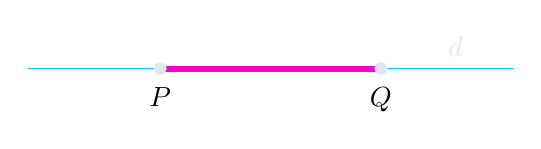
\begin{tikzpicture}[line width=1.1pt]
  \coordinate (P) at (0.6,0);
  \coordinate (Q) at (3.4,0);
  \tkzDrawLine[tmblue,add=0.6 and 0.6](P,Q)
  \draw[tmpink,line width=2.2pt] (P) -- (Q);
  \tkzDrawPoints[size=3.5,color=tminc,fill=tminc](P,Q)
  \tkzLabelPoint[below=3pt](P){$P$}
  \tkzLabelPoint[below=3pt](Q){$Q$}
  \node[tminc] at (4.35,0.28) {$d$};
\end{tikzpicture}
\end{document}
